Historical weather data has been collected for various Danish weather stations from NOAA\footnote{\url{http://www.ncdc.noaa.gov/}}. The data is in a fixed length format and contains all the necessary weather data for prediction. Format can be seen in BILAG 11111. 
The historical hourly price and wind production data has been downloaded from nordpoolspot\footnote{\url{www.nordpoolspot.com}} in excel format BILAG2.
The data will be aggregated into one file for each of the predictions containing the needed input and output parameters.

For the sake of simplicity we will be focusing on West Denmark and Funen which is also known as DK1 in the electricity market [find ref]. The collected data will be validated through plot diagrams that show and establish the relationships between weather conditions and the power generation/price of DK1.

The weather data is collected from all available weather stations in DK1 from NOAA~\ref{fig:stations4average} - some stations have been omitted due to missing data. The collected data will be averaged and used as basis for creating training sets to be used as input parameters for the Artificial Neural Networks. It is necessary to average the weather data to get a representative picture for all regions included in DK1 because only one price and production exist for all of DK1.

\begin{figure}[H]
\centering
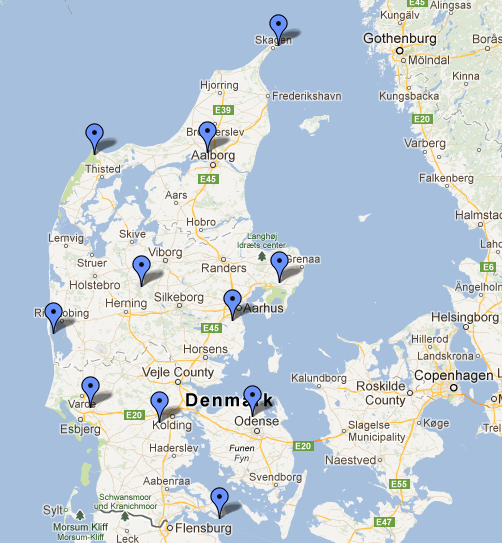
\includegraphics[width=0.85\linewidth,natwidth=898,natheight=587]{billeder/stations4average.png}
\caption{Selected weather stations in DK1}
\label{fig:stations4average}
\end{figure}


We will remove data that is obscure and is related to conditions we cannot predict. (See trimming~\ref{sec:Trimming})

we need to discuss the fact that all production data stems from nordpoolspot. The impact is obscure values a times of very low consumption. The production would not make sense in decision making if not predicted based on market conditions. The consumption will decide production together with wind speed.